%\documentclass[notes]{beamer}       % print frame + notes
%\documentclass[notes=only]{beamer}   % only notes
\documentclass{beamer}              % only frames
  \usepackage[english]{babel}
\usepackage[round]{natbib}
%\documentclass[hyperref={pdfpagelabels=false}]{beamer}
\usepackage{lmodern}
\usepackage{marvosym} % \MVRIGHTarrow

\usepackage{amsmath}  
\usepackage{multirow,graphicx,array}
\usepackage{multicol}
\usepackage{hhline}
\usepackage{xcolor}
\usepackage{colortbl}
\usepackage{threeparttable,booktabs}
\usepackage{chngcntr}
\usepackage{dcolumn}
\usepackage{caption}
\usepackage{fixltx2e}
\usepackage{rotating}




\usetheme{Singapore}
\useoutertheme{miniframes}
\AtBeginSection[]{\subsection{}}


\newcommand{\RowColor}{\rowcolor{gray} \cellcolor{white}}
\newcommand{\RowColorY}{\rowcolor{yellow} \cellcolor{white}}



\newcommand{\RN}[1]{%
  \textup{\uppercase\expandafter{\romannumeral#1}}%
}

\newcommand\Wider[2][3em]{%
\makebox[\linewidth][c]{%
  \begin{minipage}{\dimexpr\textwidth+#1\relax}
  \raggedright#2
  \end{minipage}%
  }%
}




\title{}  
\author{Monika Novackova} 
\date{September 2018} 
\institute{University of Sussex}

\setbeamercolor{block title}{bg=purple!30,fg=black}





\begin{document}


\definecolor{LightCyan}{rgb}{0.88,1,1}
\definecolor{BeigeNadine}{rgb}{1,0.94,0.86}
\definecolor{DarkGreen}{rgb}{0.1803922,0.545098,0.3411765}
\definecolor{BeigeNadine}{rgb}{1,0.94,0.86}
\definecolor{PaleGreen}{rgb}{ 0.5960784,0.9843137, 0.5960784}
\definecolor{darkblue}{rgb}{0.0, 0.0, 0.55}
\definecolor{bored}{rgb}{0.8, 0.0, 0.0}
\definecolor{babypink}{rgb}{0.96, 0.76, 0.76}

 \newcolumntype{d}{D{.}{.}{-1}}
 \newcolumntype{e}{D{+}{\,\pm\,}{6,2}}








\begin{frame}


 \begin{itemize}

     \item On average, how much does the yield change if average monthly precipitation increase by 100ml, during growing season?

 \end{itemize}
   
        
     \begin{figure}
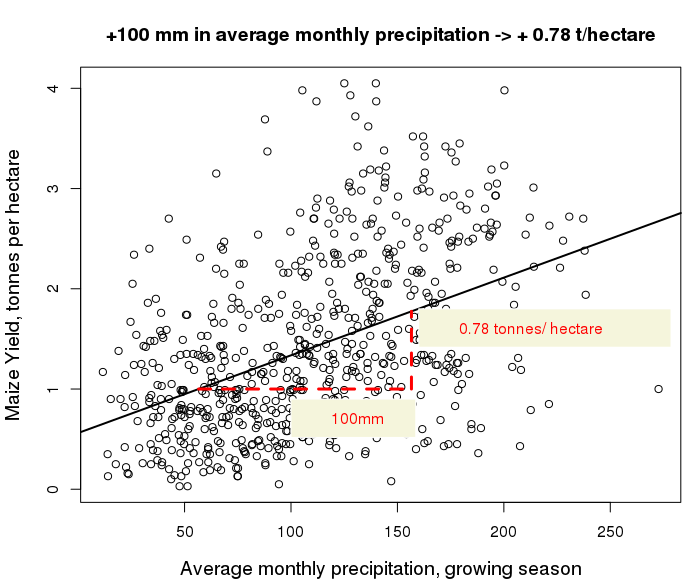
\includegraphics[width = 0.7\textwidth]{scatter.png} 
    \end{figure}
   

\end{frame}


\begin{frame}


 \begin{itemize}
     \item Models dependency of yields on weather
     
 \begin{itemize}
     \item Precipitation and weather data
        \item Growing season the most important
     
     
 \end{itemize}
          \item How reliable can we predict or estimate changes in yields based on weather data?
 \end{itemize}
   
  
      \begin{columns}
        \column{.5\linewidth }
  \begin{figure}
   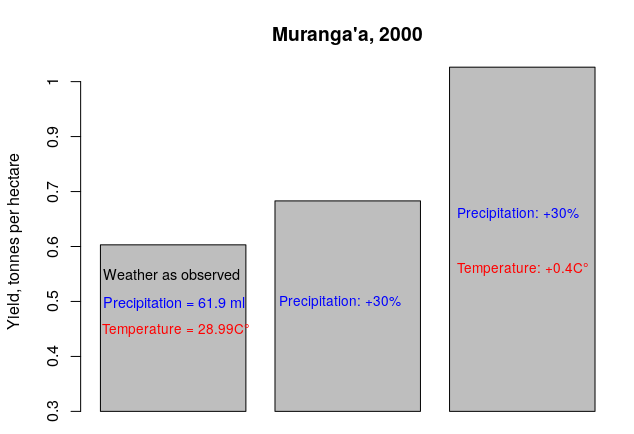
\includegraphics[width = 1\textwidth]{Muranga.png}
     \end{figure}
        \column{.5\linewidth}
           \begin{figure}
   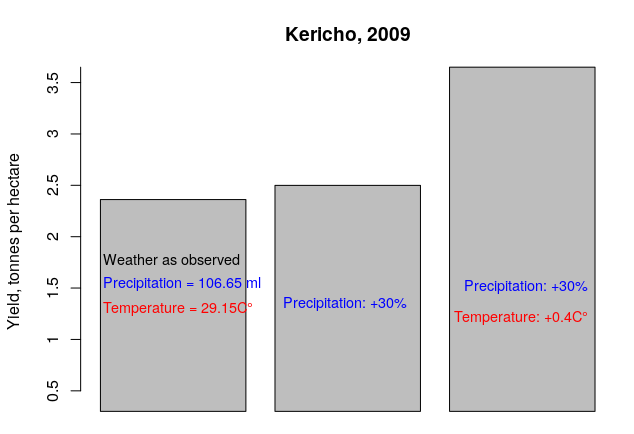
\includegraphics[width = 1\textwidth]{Kericho.png}

     \end{figure}
      \end{columns}
 



\end{frame}

\end{document}

